\documentclass[a4paper]{article}
\usepackage[utf8]{inputenc}
\usepackage[spanish, es-tabla, es-noshorthands]{babel}
\usepackage[table,xcdraw]{xcolor}
\usepackage[a4paper, footnotesep = 1cm, width=20cm, top=2.5cm, height=25cm, textwidth=18cm, textheight=25cm]{geometry}
%\geometry{showframe}

\usepackage{tikz}
\usepackage{amsmath}
\usepackage{amsfonts}
\usepackage{amssymb}
\usepackage{float}
\usepackage{graphicx}
\usepackage{caption}
\usepackage{subcaption}
\usepackage{multicol}
\usepackage{multirow}
\setlength{\doublerulesep}{\arrayrulewidth}
\usepackage{booktabs}

\usepackage{hyperref}
\hypersetup{
    colorlinks=true,
    linkcolor=blue,
    filecolor=magenta,      
    urlcolor=blue,
    citecolor=blue,    
}

\newcommand{\quotes}[1]{``#1''}
\usepackage{array}
\newcolumntype{C}[1]{>{\centering\let\newline\\\arraybackslash\hspace{0pt}}m{#1}}
\usepackage[american]{circuitikz}
\usetikzlibrary{calc}
\usepackage{fancyhdr}
\usepackage{units} 

\graphicspath{{../Ejercicio-1/}{../Ejercicio-2/}}

\pagestyle{fancy}
\fancyhf{}
\lhead{22.67 - Señales Aleatorias}
\rhead{Lambertucci, Londero B., Moriconi, Musich, Tolaba}
\rfoot{Página \thepage}

\begin{document}

%%%%%%%%%%%%%%%%%%%%%%%%%
%		Caratula		%
%%%%%%%%%%%%%%%%%%%%%%%%%

\begin{titlepage}
\newcommand{\HRule}{\rule{\linewidth}{0.5mm}}
\center
\mbox{\textsc{\LARGE \bfseries {Instituto Tecnológico de Buenos Aires}}}\\[1.5cm]
\textsc{\Large 22.67 Señales Aleatorias}\\[0.5cm]


\HRule \\[0.6cm]
{ \Huge \bfseries Trabajo práctico N$^{\circ}$3}\\[0.4cm] 
\HRule \\[1.5cm]


{\large

\emph{Grupo 1:}\\
\vspace{3pt}

\begin{tabular}{lr} 	
\textsc{Lambertucci}, Guido Enrique  & 58009 \\
\textsc{Londero Bonaparte}, Tomás Guillermo  & 58150 \\
\textsc{Musich}, Francisco  & 58124\\
\end{tabular}

\vspace{20pt}

\emph{Profesor}\\
\textsc{Hirchoren}, Gustavo Abraham \\
\vspace{3pt}
%\textsc{} \\	

\vspace{100pt}

\begin{tabular}{ll}

Presentado: & 07/02/22\\

\end{tabular}

}

\vfill

\end{titlepage}


%%%%%%%%%%%%%%%%%%%%%
%		Indice		%
%%%%%%%%%%%%%%%%%%%%%

\tableofcontents
\newpage

%%%%%%%%%%%%%%%%%%%%%
%		Informe		%
%%%%%%%%%%%%%%%%%%%%%


\subsection{Introducción}

Se analiza una secuencia $X(n)$ de 32768 muestras, estimando y calculando parámetros de interés, como lo son la autocorrelación, los coeficientes de correlación parcial, a partir de estos se generará un modelo AR con el propósito de ajustar dicha serie, y con los coeficientes autoregresivos diseñar un modelo en variables de estados del sistema para utilizar un filtor de Kalman.\\
A la secuencia se le agregará ruido blanco gaussiano aditivo (AWGN) para simular el ruido de medición.\\
Cabe destacar que en este informe se hará referencia a una variable p, esta tiene un rango entre 1 y 9.\\

\subsection{Estimación de la Autocorrelación} 

Se estiman la autocorrelación mediante el uso de los primeros p elementos de la secuencia brindada. Para ello, se vale del  no polarizados ($R_{np}$) de dicho parámetro. Esta funcion es  empleadas para estimar otras funciones mediante información digitalizada.
\begin{equation}
\begin{gathered}
	R_{np}(k) = \frac{1}{N-k} \sum_{i=0}^{N-k-1} X(i)X(i+k)
\end{gathered}
\end{equation}


\begin{figure}[H]
\centering
	
\includegraphics[width=0.8\textwidth, trim = {0 0 0 0},clip]{./Imagenes/pend.jpg}
	\caption{Grafica de los coeficientes de autocorrelación total estimados.}
	\label{fig:rxx}
\end{figure}



\subsection{Coeficientes de correlación parcial}

Con los datos ya extraídos y mediante la resolución de la ecuación de Yule-Walker, fue posible obtener los coeficientes deseados. Esto se realizó con los coeficientes totales obtenidos a través de la estimaciones no polarizada, para cada p se obtiene un vector de tamaño $\left[ 1 \ \times \ p \right]$ que corresponde a los $\phi_{p,i}$.
\begin{figure}[H]
\centering

	
\includegraphics[width=0.7\textwidth, trim = {0 0 0 0},clip]{./Imagenes/pend.jpg}
	\caption{Coeficientes de correlación parcial a partir de la matriz de Yule Walker.}

	\label{fig:phikk}
\end{figure}

Cabe destacar que en ningun caso los coeficcientes de correlacion parcial se hacen nulos, por lo que no hay seguridad de que un modelo Auto Regresivo se ajuste a la secuencia.
\subsection{Modelo del proceso}
\label{subsec:modelo}

El tipo de modelo a utilizar para el proceso será un Auto Regresivo, se utilizará un AR(p). .

Para el calculo de los $\phi$, son los obtenidos de la matriz de Yule Walker
\begin{equation}
Ecuacion \ de \ yule \  walker
\end{equation}


\begin{figure}[H]
\centering

	
\includegraphics[width=0.8\textwidth, trim = {0 0 0 0.},clip]{./Imagenes/pend.jpg}
	\caption{Grafico relevante.}

	\label{fig:Rxxcalc}
\end{figure}


\subsection{Filtro de Kalman}
El filtro de Kalman es un filtro adaptativo recursivo el cual consiste en...
\begin{figure}[H]
\centering

	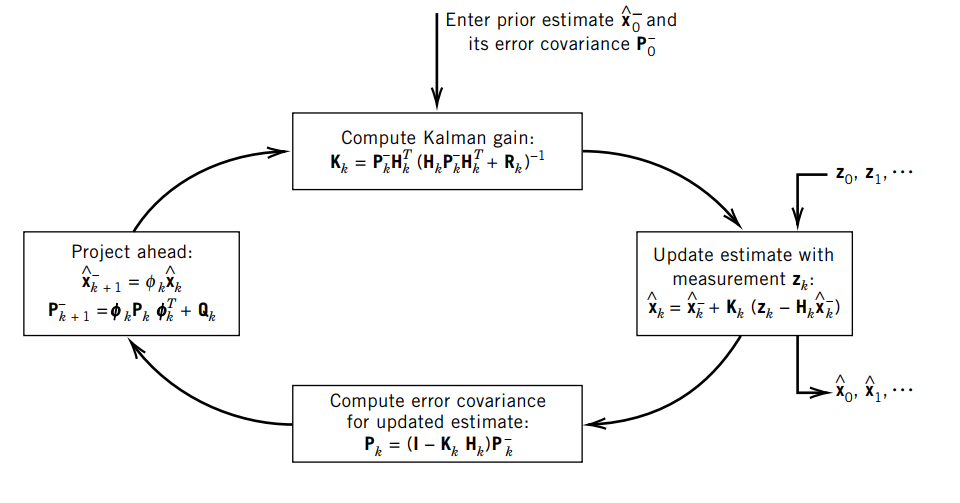
\includegraphics[width=0.8\textwidth, trim = {0 0 0 0},clip]{./Imagenes/kalman_loop.png}
	\caption{Iteración del filtro de Kalman.}
	\label{fig:Kalman_loop}

\end{figure}

\subsubsection{Modelo en variables de estado}
Aca explico las matrices y el modelo estas cosas de \LaTeX esta bien piola
\begin{equation}
\underset{n\times 1}{\mathrm{Y}} =  \underset{n\times p}{X} \times 
\underset{p\times 1}{\theta} + \underset{n\times 1}{\varepsilon}
\end{equation}

\subsubsection{Implementacion del filtro recursivo}

\begin{figure}[H]
\centering
	
\includegraphics[width=0.8\textwidth, trim = {0 0 0 0.735cm},clip]{./Imagenes/pend.jpg}
	\caption{Periodigramas obtenidos a partir de las estimaciones de $R_{XX}$.}
	\label{fig:period-est}
\end{figure}

\subsection{Análisis de resultados}
El mierdas comparativo con gráficosa
\subsection{Código implementado}
El mierda.m
\begin{itemize}
\item Main.m:
	\lstinputlisting[language=Matlab]{../Matlab/Main.m}
	
\item Cpar.m:
	\lstinputlisting[language=Matlab]{../Matlab/cpar.m}
	
\item Rnp.m:
	\lstinputlisting[language=Matlab]{../Matlab/Rnp.m}
	
\item kalman.m:
	\lstinputlisting[language=Matlab]{../Matlab/kalman.m}

\end{itemize}

\end{document}